\documentclass{article}
\usepackage[T2A]{fontenc}
\usepackage[english, russian]{babel}

\begin{document}

\title{Изучение предметно следственных связей в естественном языке посредством графовых вероятностях моделей для адаптации к большим языковых моделей}

\section{Предисловие}

Научные знания имеют высокую ценность для развития общества и самореализации личности.
Постиндустриального общества ориентировано на инновационный сектор с постоянной потребностью
в нововведениях и улучшению устоявшихся процессов. Ключевыми условиями  поддержания 
такого общества является повсеместное стремление к профессиональному росту, расширению компетенций
и непрерывное образование на протяжении всей жизни. 

Тем не менее структура научного знания преимущественно ориентирована на специалистов, что осложняет его
персональное освоение. В современной реальности существует два основных подхода к обучению: специализированные курсы
и прохождение образовательной программы в высшем образовательном учреждении. Оба подходы 
имеют обоснованную пользу для работы, требующих
специальной подготовке и перенятая опыта у предметного специалиста. Тем не менее
профессиональное обучение как правило подготавливает специалистов с глубокими знаниями лишь в одной сфере.
Тем не менее в условиях высококонкурентного российского рынка востребованы
интеллектуальные продукты, адаптирующиеся под изменчивые потребности конечного потребителя.
В современных реалиях от предметного специалиста ожидаются навыки введения организации, 
правового оформления деятельности и разработки интерфейса сетевого взаимодействия. 

Как правило, отсутствие даже одного из этих навыков приводит к краху 
трудовой инициативы, поэтому их освоение проходит комплексно в и вне рабочего времени. 
Обучение проходит преимущественно персонально через критическое 
осмысление корпусов текстов. Целью деятельности является построение 
таксономического древа определений и сопоставления практической постановки с модельно описанной. 
Вследствие пересеченности научных дисциплин сложность задачи повышается потребностью декомпозиции предметных постановок
на известные области знаний. 

Сбор корпуса выполняется через системы информационного поиска, выделяющие документы через
ключевые слова и ссылки. Такой подход осложняется невозможностью в явной форме получить ответ на вопрос.  
Автоматические интеллектуальные ассистенты во многом разрешают проблемы, но даже приближающиеся к человеческим способностям
большие языковые модели не способны на формальные логические операции: арифметического сложения, решения абстрактных логических задач, соблюдение 
правил стратегических игр.

Одним из возможных путей разрешения являются графовые модели знаний, основанные 
на байесовых сетях. \footnote{Альтернативный подход заключается в обучение языковой модели работе с инструментами. Таковыми могут быть калькуляторы,
языки программирования или поисковые инструменты.} Такие сети представляют представляют связь между понятиями вероятностно, 
задавая причинно-следственный аппарат как направление в ребре связи графа. 
Итоговая модель представляет собой статистическую модель явления, которую можно использовать для
управления и анализа системой. 

Описанный подход называется \textit{вариационным причиннно-следственным выводом}. Направление развивается на стыке логики,
теории алгоритмов и графового анализа. Разработанные модели применяются в  
Автор видит большой потенциал в заданных моделях и 

\section{Предметный обзор направления исследования}

\subection{Введение}

Графовое представление позволяет разрешать мысленные парадоксы причинности.

\begin{figure}[h]
    \centering
    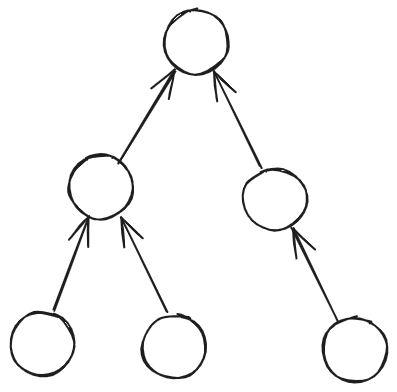
\includegraphics[width=0.5\textwidth]{assets/graph.excalidraw.png}
    \caption{Графовое представление}
    \label{graph}
\end{figure}





Таким образом, проведенный анализ позволяет судить о достоверности суждений и том, как именно их нужно изменить 
для получения более

Зададим ключевые предметные определения.

\subsection{Направление исследования} 


Формально опишем заданные в предисловия пожелания к аппарату вероятностных графовых моделей.


\begin{figure}[h]
    \centering
    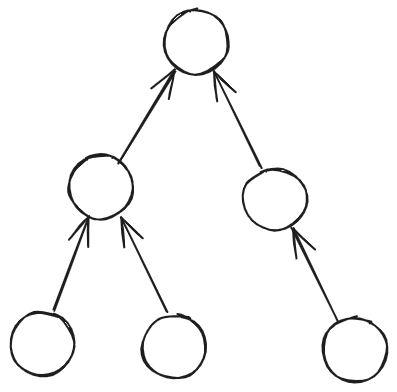
\includegraphics[width=0.5\textwidth]{assets/graph.excalidraw.png}
    \caption{Графовое представление}
    \label{graph}
\end{figure}

\subsection{Изучение причинно-следственные связи}



Таким образом порождающая дискриминативной модели являются возможность порождения.


\textit{Определение} Графовой вероятностная модель называется граф $\Gamma = (E,V)$, где для каждого 

Графовые модели принципиально различаются на марковские поля
\footnote{термин поля связан с определенными операциями сложения и ренормализации формально соотвествующим требованиям поля}
и байесовы сети \cite{lafferty2001conditional}.


\begin{figure}[h]
    \centering
    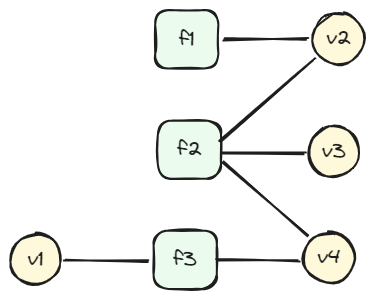
\includegraphics[width=0.5\textwidth]{assets/factor_graph.excalidraw.png}
    \caption{Фактор-граф представляет}
    \label{graph}
\end{figure}


\subsection{Выбор оптимальной модели}


Выбор топологии графа выполняется по принципу Оккаме: граф должен быть прост, но исчерпывающе описывать постановку. Для этого
все параметры модели согласно байесовскому подходу задаются случайными величинам с известными статистическими распределениями.М
После сравнивая маргниальную вероятность всех возможных форм граф находится наилучшая конфигурации $\Gamma$. Такой подход, в общем
случае требует значительных вычислительных ресурсов, поскольку маргинализация является NP-полной задачей, экспоненциально усложняющейся
с числом роста фактором.

Обновление представлений 

Алгоритмы выполняющий расчет


\subsection{Байесовы сети}

Для байесовых сетей 

\begin{figure}[h]
    \centering
    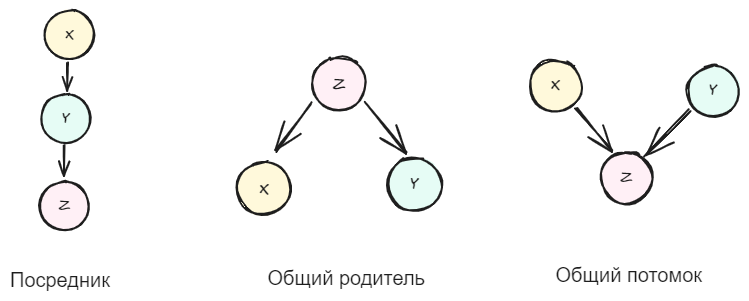
\includegraphics[width=0.5\textwidth]{assets/bayes_net.excalidraw.png}
    \caption{Элементарными структурами байесовых сетей являются группы }
    \label{bayes-net}
\end{figure}


\subsubsection{Вариационный причино-следственный анализ}

Ключевым для анализа полученного графа является понятие потока зависимостей, задающего связь между наблюдаемой и инструментальными переменными.
Задача специалиста найти способ на заданных данных свести многокомпонетный анализ, осложненный учетом
взаимного влияния факторов друг друга, к изучения влияния одного признака. Такая задача, как правило, выполняется через 
фиксации прочих признаков через зависимые. 

\textit{Определение} (от \texit{англ. cofounder} ) 


\textit{Определение} \textit{Интервенция} называется


\subsubsection{Техники}

Причинно-следственной связь

Оптимизация графовой модели выполняется посредством аггрегации сообщений соединненых ребер.

\begin{figure}[h]
    \centering
    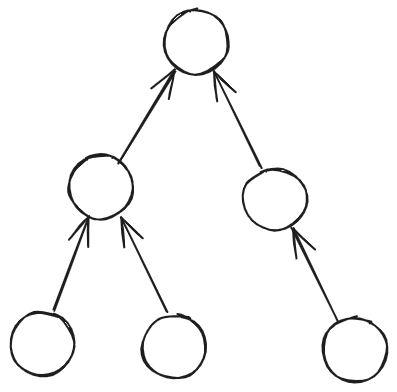
\includegraphics[width=0.5\textwidth]{assets/graph.excalidraw.png}
    \caption{Таксономия современных подходов обработки естественного языка}
    \label{llm_taxonomy}
\end{figure}



\section{Теоретический аппарат}




Аналитическое исследование причинно-следственных связей на данных выполняется с помощью генеративных графических моделей.

Для анализа используются маргни



Принципиально рассчитывается вероятность заданной цепочки логических рассуждения .
Опишем постановку более формально с введением и ключевых понятий и пояснением метода оптимизации. 

\textit{Определение} Вероятностная модель называется графовой, если ребра графа

Каждое ребро графа имеет вероятностную модель $P(X|A)$, в простейшем случае представленную ло

Таким образом, граф с наибольшей вероятностью является. 

\begin{equation}
    x^t_{i+1} = x_i + f(x_1, \dots, x_n), 
\end{equation}

$$
    \lambda_n  f(x_1, \dots, x_n), 
$$


\texit{Определение} Случай дерево

\section{Научно-образовательная деятельность автора}

\subsection{Изданные работы}




Супераддитивной называется функция $f$ для которой
\begin{equation}
    \forall x, y, x+y \in \text{dom}(f) \rightarrow f(x+y) \ge f(x) +f(y) 
\end{equation}

Для квадратичной формы 

\begin{equation}
    \begin{aligned}
        & \mathbb{E}[\varepsilon^T \Lambda \varepsilon] = \operatorname{tr}[\lambda] \\ 
        \var\[\\]
    \end{aligned}
\end{equation}


Такие функции позволяю оценить по индивидуальным качествам учащихся их совместный вклад в дело. Примерами супераддитивных функций являются \begin{itemize}
    \item min-sum $\sum_{i} min([\vec{x}]_i,s^*)$, гдe $s^*$ - порог отсечки
    \item max-mean $N \cdot \bar{x} + \max_i(\vec{x} - \bar{x})$
    \item квадратичная форма $\vec{x}^T A \vec{x}$
\end{itemize}

\begin{figure}[h]
    \centering
    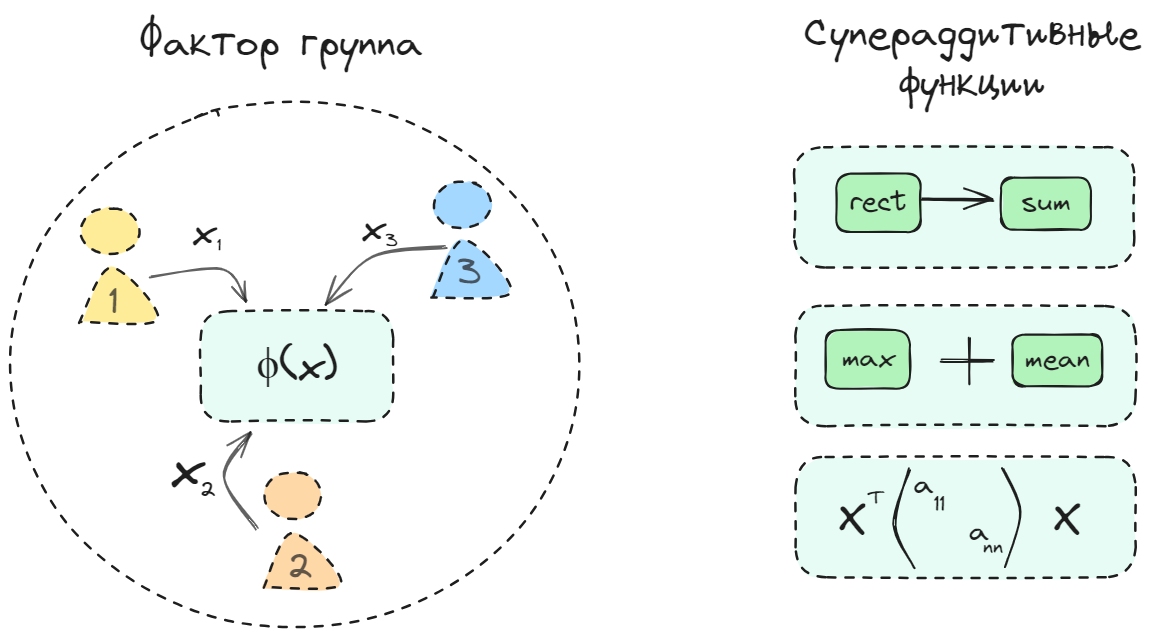
\includegraphics[width=0.5\textwidth]{assets/final/group.excalidraw.png}
    \caption{Групповые задания}
    \label{group_task}
\end{figure}

Учет коллективных эффектов
выполняется в постановках распределенной оптимизации, теории марковских полей и теоретической физике. Для анализа взаимодействия в группах малых групп используются 
ковариационные матрицы. 


Совместное обучение подразумевает одновременное достижение высоких уровней компетенций в предмете изучения.
Такое обучения, как правило, сопровождается подготовленным методическими материалами общими для всех обучающихся.
Задача преподавателя в наиболее успешном прохождение учащихся методической программы. При внесении изменений
в курс оценивается изменение среднего показателя учащихся. Усредненные аналитические показатели позволяют принимать решения с статически заданными
порогами риска и приобретений. Это обеспечивает устойчивые рост образования в среднем. Для развития практики
полезно учитывать индивидуальные потребности учащихся, заключающиеся в разном уровне освоения материала и задачах его использования. Разрешить проблему
можно путем индивидуального образования, но такой подход осложнен увеличением преподавательской нагрузки. Одним из компромиссных решений является групповое образование,
обеспечивающее баланс между специфичностью задания для учащегося и временем для проверки для преподавателя.



Практически функцию улучшение среднего результата в классе. 


\begin{figure}[h]
    \centering
    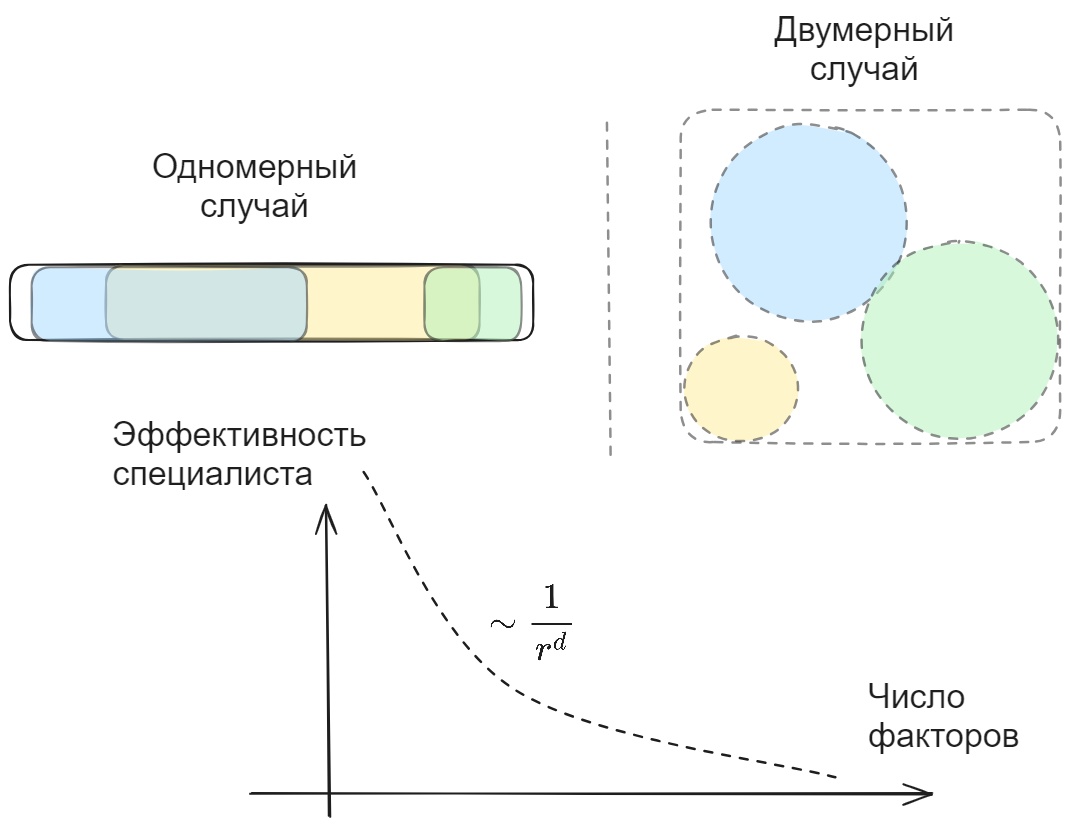
\includegraphics[width=0.5\textwidth]{assets/final/geometry.excalidraw.png}
    \caption{Групповые задания}
    \label{group_task}
\end{figure}


Общий результат лучше исключает
случайности и может быть оценкой эффективности как отдельного педагога, так и всего преподавательского коллектива.
Тем не менее такой подход не всегда может учесть индивидуальные образовательные потребности учащихся. Одним из возможных
разрешений такой проблемы является объединение учащихся в группы для выполнения задач.






\end{document}




